\documentclass{beamer}
\usefonttheme[onlymath]{serif}
\usepackage{amsmath}
\usepackage{amsfonts}
\usepackage[export]{adjustbox}
\usepackage[utf8]{inputenc}

% definitions
\def\H{\mathcal{H}}
\def\X{\mathbf{X}}
\def\w{\mathbf{w}}
\def\W{\mathbf{W}}
\def\const{\mathrm{const}}
\def\Var{\mathrm{Var}}
\def\tr{\mathrm{tr}}
\def\T{\top}
\def\U{\mathbf{U}}
\def\S{\mathbf{S}}
\def\V{\mathbf{V}}
\newcommand{\argmin}{\mathop{\mathrm{argmin}}}
\newcommand{\argmax}{\mathop{\mathrm{argmax}}}
\newcommand{\minimize}{\mathop{\mathrm{minimize}}}
\newcommand{\maximize}{\mathop{\mathrm{maximize}}}
\newcommand{\st}{\mathop{\mathrm{subject\,\,to}}}

%Information to be included in the title page:
\usecolortheme{seahorse}
\title{Occam's Razor}
\author{Thomas Bayes}
\institute{
\includegraphics[height=.3\textheight]{../bayes.png}%
}
\date{\today}

    
    
\begin{document}
    
\frame{\titlepage}

\begin{frame}{Question}
How many boxes are behind the tree? One or two?
\begin{center}
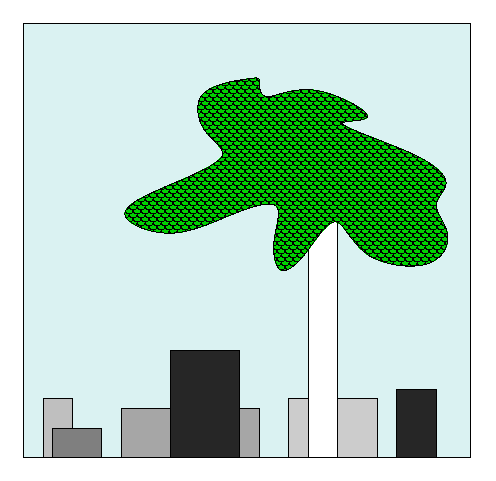
\includegraphics[scale=0.8]{./figure196.eps}
\end{center}
\end{frame}

\begin{frame}{Occam's Razor}
\begin{itemize}
\item \textit{Accept the simplest explanation that fits the data.}
\item \textit{Plurality is not to be posited without necessity.}
\item \textit{Less is more.}
\end{itemize}
The intuition maybe is 'well, it would be a remarkable \textbf{coincidence} for the two boxes to be just the same height and colour as each other.'
\end{frame}
    
\begin{frame}{Bayesian derivation of Occam's Razor}
We have two hypothesis $\H_1$ and $\H_2$. We are interested in the posterior of $\H_1$ and $\H_2$ in light of data $D$. 
$$\frac{P(\H_1 | D)}{P(\H_2 | D)} = \frac{P(\H_1 | D)}{P(\H_2 | D)}\frac{P(D|\H_1)}{P(D|\H_2)}$$
The first part is our preference of the one-box or two-box hypothesis. In this case, it seems quite natural to say we have no prefrences over the number of boxes(Note that Occam's Razor principle does not apply here, because one-box hypothesis does not necessarily mean simpler.)
\end{frame}
\begin{frame}{One box or two box?}
Our two-box hypothesis will lay wider distribution on the space, thus the \textit{particular data} we are observing will share lower probablity.
\begin{center}
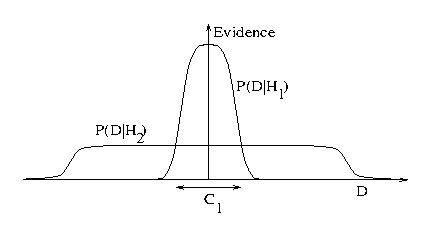
\includegraphics[scale=1]{./figure197.eps}
\end{center}
\end{frame}

\begin{frame}{Number example}
\begin{tabular}{cl}  
\begin{tabular}{c}
\includegraphics[scale=0.3]{./number-example.jpg}
\end{tabular}
& \begin{tabular}{l}
\parbox{0.5\linewidth}{%  change the parbox width as appropiate
In this example (extracted from online), we have two hypothesis, $\H_1$: the sequence is an arithmetic progression, $\H_2$: the sequence is generated from a fourth-order polynomial.\\
One possible reason for our preferences over $\H_1$ is maybe, in our mind, we think a sequence is more likely to be generated from arithmetic progressio, so $P(\H_1) > P(\H_2)$. \\
And another reason is that it is less likely for a fourth-order polynomial to somehow accidently generate four integer numbers!
}
\end{tabular}  \\
\end{tabular}
\end{frame}
\begin{frame}{References}
Chapter 28 of \textit{Information Theory, Inference, and Learning Algorithms} by  \textbf{David J.C. MacKay}
\end{frame}
\end{document}